\chapter{Ví dụ minh họa với NodeJS}
\label{Ví dụ minh họa với NodeJS}

Trong phần này, ta hãy cùng tìm hiểu một ứng dụng chat đơn giản. Mã nguồn của chương trình có thể tìm thấy tại địa chỉ:\\
	\url{http://github.com/}\\
Cấu trúc chương trình được thể hiện qua hình dưới đây:\\
	\begin{figure}[-h]
		\centering
		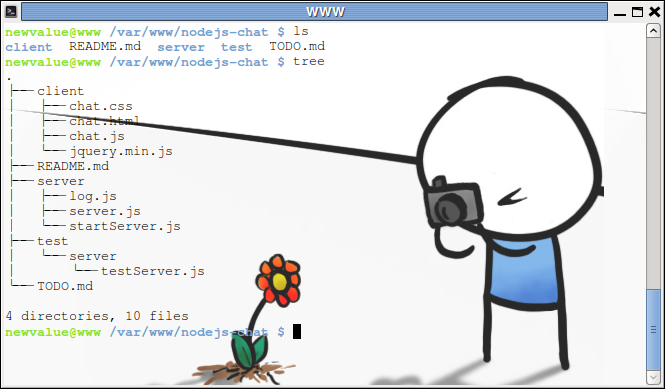
\includegraphics[scale=0.7]{4_1}
	\end{figure}
	
	\begin{tabular}{|c|c|}
		\hline
		Tên file/Thư mục & Miêu tả \\
		\hline
		Client & Thư mục hiển thị ngươi dùng \\
		\hline
		client/server.js & Quản lý giao tiếp giữa client và server \\
		\hline
		Server/ & Chứa mã nguồn server \\
		\hline
		Server/server.js & Module Server \\
		\hline
		server/log.js &	Module log: quản lý thông báo, ghi chép \\
		\hline
		server/startServer.js &	Tạo một thể hiện của server và chạy \\
		\hline
		test/server/test.js & Test \\
		\hline
	\end{tabular}
	
\section{Module Server}
	Đây là module chính của chương trình.Nhiệm vụ của nó là khởi tạo một server lắng nghe và phản hồi các kết nối.\\
	Trong ví dụ này, để thực hiện kết nối giữa server và client, ta sẽ sử dụng WebSocket – một công nghệ mới cho phép tạo các luồng socket trên nền HTTP. Do vậy tta phải khởi tạo một TCP Server:\\
	\begin{minted}[linenos=true, frame=single]{javascript}
this.server = tcp.createServer(function(socket){

});
	server.listen(7000);
	\end{minted}
	
	Để có thể quản lý các kết nối từ client, ta tạo một mảng lưu trữ lại các kết nối.\\
	\begin{minted}[linenos=true, frame=single, tabsize=4]{javascript}
this.connections = []
...
var self = this;
this.server = tcp.createServer(function(socket){
	var connection = new module.Connection(self, socket);
	self.addConnection(connection);
});
	
this.addConnection = function(connection){
	self.connctions.push(connection);
	connection.id = self.nextIdAssign++;
}
	\end{minted}
	
	Khi có một yêu cầu từ phía client gửi đến, ta sẽ gửi broadcast các tin nhắn tới các user khác:\\
	\begin{minted}[linenos=true, frame=single, tabsize=4]{javascript}
//gui tin nhan tu client
this.say = function(){
	self.broadcast(function(conn){
		return ['said', {
			'is self': (conn.id == connection.id),
			'message': message,
			'nick': connection.nick
		}
	});
};
//broad cast
this.broadcast = function(fn){
	self.connection.each(function(connection){
		var data = fn(connection);
		connection.send(data);
	}
}
	\end{minted}
	
Khi client gửi yêu cầu hủy kết nối, ta phải loại bỏ kết nối của client ra khỏi danh sách kết nối:\\
	\begin{minted}[linenos=true, frame=single, tabsize=4]{javascript}
this.removeConnection = function(connection){
	self.connection.remove(connection);
	log.debug('Connection: ' + self.connections.length);
}
	\end{minted}
	
Bây giờ ta cùng xét đên lớp kết nối. Mục đích lớp này để quản lý kết nối. Một thể hiện của lớp này cần lưu trữ thông tin server quản lý nó, socket, id và nick đang kết nối tới. Id này do lớp Server đánh số. Trước hết nó được dùng để gửi lại tin nhắn do server nhận được ở trên.\\
	\begin{minted}[linenos=true, frame=single, tabsize=4]{javascript}
this.send = function(){
	try {
		//chuyen mang dữ liệu data sang xau json
		self.socket.send('\u0000' + JSON.stringfy(data)  + '\uffff');
	}catch(e){
		//ngat ket noi khi co loi
		//self.disconnect();
	}
}
	\end{minted}

	Ngoài ra trong ví dụ này, ta sẽ cho phép người dùng đăng ký tên để sử dụng. Để tiện cho việc này, ta viết thêm phương thức quản lý yêu cầu. Ta sẽ quản lý 2 loại yêu cầu:
	\begin{itemize}
		\item Đăng ký nick
		\item Gửi nhận tin nhắn
	\end{itemize}
	
	\begin{minted}[linenos=true, frame=single, tabsize=4]{javascript}
this.Connection.prototype.handlers = {
	assignNick: function(connection, data) {
		log.debug(connection.logFormat('Assigning nick: ' + data));
		connection.nick = data;

		connection.send(['lastMessage', connection.server.lastNMessages(5)]);
		connection.server.broadcast(function(conn) {
			return ['status', { 'nick': connection.nick, 'status': 'on' }];
		})
	},

	say: function(connection, data) {
		connection.server.say(connection, data);
	}
};
	\end{minted}


\section{Module Client}
Để thực hiện kết nối với server ta sẽ sử dụng WebSocket để tạo một socket yêu cầu tới  server:
	\begin{minted}[linenos=, tabsize=4. frame=single]{javascript}
NodeJSChat.ws = new WebSocket('ws://localhost:7000')
NodeJSChat.ws.onmessage = NodeJSChat.onmessage;
NodeJSChat.ws.onclose = NodeJSChat.onclose;
NodeJSChat.ws.onopen = NodeJSChat.onopen;
	\end{minted}

Từ đó ta sẽ xây dựng các hàm callback tương ứng với từng sự kiện:\\
	\begin{minted}[linenos=true, frame=single, tabsize=4]{javascript}
,

	onclose: function() {
		NodeJsChat.debug('socket closed');
		if (!NodeJsChat.windowClosing) {
			alert('Whoops! Looks like you lost internet
			connection or the server went down');
    }
},
	\end{minted}
	
	\begin{minted}[linenos=true, frame=single, tabsize=4]{javascript}
onmessage: function(evt) {
	var jsonData = JSON.parse(evt.data);

    var action  = jsonData[0];
    var data    = jsonData[1];

    if (NodeJsChat.handlers[action]) {
      NodeJsChat.handlers[action](data);
    }
    else {
      // This should be in a separate function.
      $('#messages').append('<tr><td cospan="2">Whoops, bad message
					from the server</td></tr>');
    }
},

onopen: function() {
    NodeJsChat.debug('Connected...');
    NodeJsChat.send([ 'assignNick',  NodeJsChat.nick ]);
},
	\end{minted}

Khi người dùng nhấn gửi tin, ta sẽ sử dụng socket này để gửi tới server:
	\begin{minted}[linenos=true, frame=single, tabsize=4]{javascript}
say: function(message) {
	NodeJsChat.send([ 'say',  message ]);
    return false;
},

send: function(data) {
	var dataStr = JSON.stringify(data);
    NodeJsChat.ws.send(dataStr);
},
	\end{minted}

Cuối cùng, ta xây dựng một phương thức điều khiển chung cho mọi yêu cầu từ client.Các yêu cầu gồm có:
	\begin{itemize}
		\item Cập nhật các tin nhắn gần nhất.
		\item Ghi nhận trạng thái hiện tại.
	\end{itemize}

	\begin{minted}[linenos=true, frame=single, tabsize=4]{javascript}
said: function(data) {
	var message = '<div class="message">';

    var prefix  = '';
    var tdClass = '';
    if (data.isSelf) {
      prefix  = 'You:';
      tdClass = 'me';
    }
    else {
      prefix  = data.nick + ':';
      tdClass = 'nick';
    }
    message     += '<div class="' + tdClass + '">';
    message     += prefix
    message     += '</div>';

    message     += '<div class="message">';
    message     += data.message;
    message     += '</div>';

    message     += '</div>';

    $('#messages').append(message);
  },

  status: function(data) {
    var nick = data.nick;
    var stat = data['status'];

    var message = '<div class="status">' + nick 
    		+ ' just logged ' + stat + '</div>';
    $('#messages').append(message);
  }
};
	\end{minted}
